\documentclass[../../main.tex]{subfiles}

\graphicspath{{\subfix{../../immagini/}}}

\begin{document}

I metodi introdotti negli scorsi paragrafi, come già accennato, risultano in molti contesti fortemente limitati nel tipo di pattern che possono descrivere, per questo motivo si rendono necessari modelli più \textit{espressivi} per poter approssimare le funzioni più complesse.

Introduco quindi ora il concetto di \textit{rete neurale artificiale} e mi concentro poi su due specifiche \textit{architetture} di reti: \textit{percettroni multistrato} e \textit{reti ricorrenti}, che saranno quelle utilizzate negli esperimenti descritti nei capitoli successivi.  

Formalmente una \textit{rete neurale} è una tripla $(N, V, w)$ dove $N$ rappresenta l'insieme di neuroni della rete, $V$ è un insieme della forma $\{(i, j) \ | \ i,j \in \mathbb{N} \}$ e rappresenta le \textit{connessioni} tra le unità della rete $i$ e $j$, infine $w$ è una funzione definita come:
\[w : V \rightarrow \mathbb{R}\]
che rappresenta il \textit{peso} di una connessione $(i, j)$. \cite{kriesel2007bin}

Una rete è quindi formata da unità computazionali, dette \textit{neuroni}, collegate tra loro da \textit{connessioni} caratterizzate da un \textit{peso}, che intuitivamente rappresentano la forza di una connessione.

\begin{figure}[H]
    \centering
    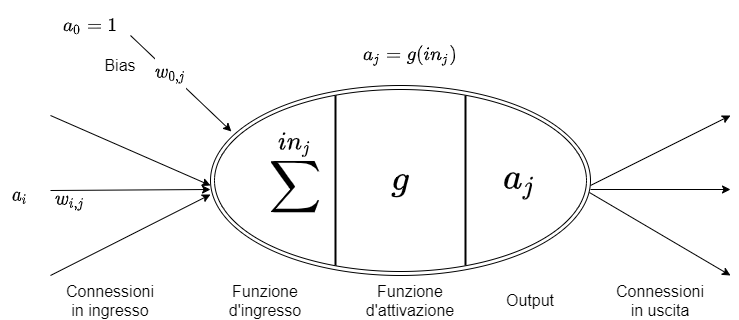
\includegraphics[width=\textwidth]{immagini/4_2/neuron.png}
    \caption{Struttura di un neurone}
    \label{fig:neuron}
\end{figure}

Ogni neurone risulta collegato con una serie di altre unità ricevendo in ingresso i rispettivi output che trasforma in base al valore dei relativi pesi $w_{i,j}$, una volta prodotto l'output questo viene a sua volta \textit{propagato} ad una serie di altre unità funzionali.

Formalmente posso suddividere la struttura di un neurone in diverse parti (Figura \ref{fig:neuron}): ogni valore ricevuto in ingresso prende il nome di \textit{attivazione} $a_i$, questi vengono prima passati attraverso una funzione d'ingresso, che spesso viene definita come somma \textit{pesata} dei valori d'ingresso:
\[in_j = \sum_{i=0}^n {w_{i,j} a_i}\]
Il risultato della funzione d'ingresso viene poi fornito in input alla \textit{funzione d'attivazione} $g$:
\[a_j = g(in_j) = \sum_{i=0}^n {w_{i,j} a_i}\]
Infine il valore d'attivazione viene passato attraverso una \textit{funzione di output} che spesso semplicemente corrisponde ad una funzione identità:
\[f_{out}(a_j) = a_j\]
Il valore $a_j$ prodotto viene poi propagato ai neuroni dei livelli successivi ed il processo appena descritto viene ripetuto fino ad arrivare allo strato d'uscita.

In generale la funzione d'attivazione può avere diverse forme:

\begin{figure}[H]
    \centering
    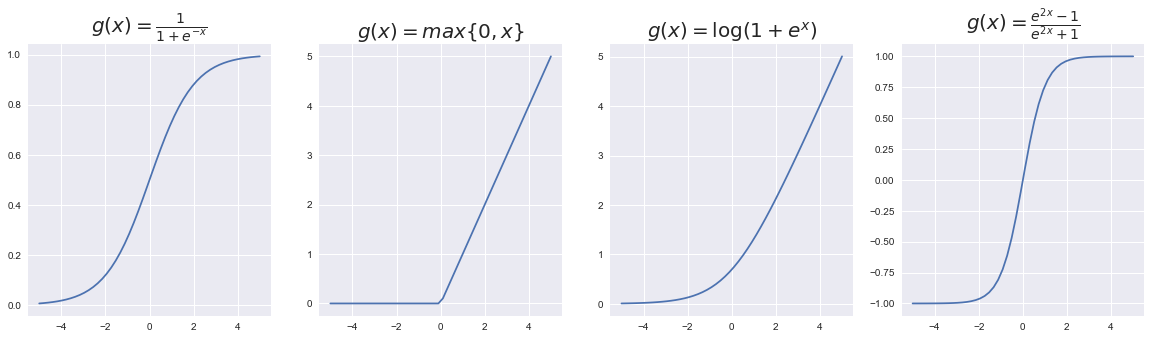
\includegraphics[width=\textwidth]{immagini/4_2/activation_func.png}
    \caption{Esempi di tipiche funzioni d'attivazione}
    \label{fig:activations}
\end{figure}

L'aspetto che rende le reti neurali modelli in genere più espressivi rispetto ad approcci come regressione lineare o logistica, definiti nei paragrafi precedenti, è il fatto di poter connettere più unità funzionali tra di loro, in questo modo l'uscita può essere descritta da una espressione che ha la froma di una funzione innestata:
\[f_k\left(f_{\dots}\left(f_2\left(f_1(\boldsymbol{x})\right)\right)\right)\]

Per "sfruttare" a pieno questa caratteristica è però importante che la funzione d'attivazione sia:
\begin{itemize}
    \item \textit{Non lineare}: altrimenti l’uscita della rete sarebbe sempre lineare e il modello sarebbe troppo semplice.
    \item \textit{Differenziabile}: su buona parte del dominio e monotona non decrescente, per poter facilitare la applicazione di algoritmi basati sulla discesa del gradiente.
\end{itemize}
Nel caso in cui $g$ sia una funzione a soglia (Figura \ref{fig:threshold}) parlo di \textit{percettrone}.

Una volta definita la struttura di un neurone è utile analizzare il come questi possono connettettersi per andare a formare la rete: le due tipologie di \textit{architetture} utilizzate negli esperimenti sono la \textit{rete feed forward} (Figura \ref{fig:feedforward}) e la \textit{rete ricorrente} (Figura \ref{fig:RNN})

\begin{figure}[H]
    \begin{subfigure}[]{0.48\textwidth}
        \centering
        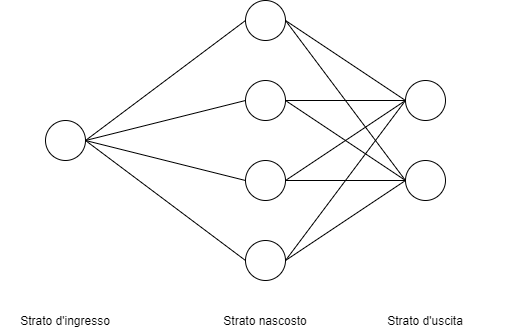
\includegraphics[width = \textwidth]{immagini/4_2/feed_forward.png}
        \caption{Esempio di rete neurale con architettura feed forward}
        \label{fig:feedforward}        
    \end{subfigure}
    \begin{subfigure}[]{0.48\textwidth}
        \centering
        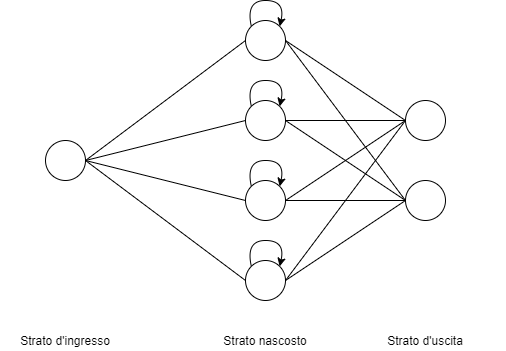
\includegraphics[width = \textwidth]{immagini/4_2/RNN.png}
        \caption{Esempio di rete neurale ricorrente, in questo caso la ricorrenza è solamente diretta}
        \label{fig:RNN}
    \end{subfigure}
\end{figure}

Una \textit{rete feedforward} è composta da un livello d'ingresso e da un livello d'uscita e da uno o più livelli nascosti. Le connessioni in questa topologia sono permesse solo tra neuroni di livelli consecutivi.\\
Se il numero di livelli nascosti è superiore a 3 si parla di \textit{reti profonde}.

Una \textit{rete ricorrente} è un topologia in cui sono permesse interconnessioni tra neuroni che generano cicli: parlo nello specifico di ricorrenza \textit{diretta} nel caso in cui un neurone sia connesso con sé stesso, di ricorrenza \textit{indiretta} quando sono ammesse connessioni verso livelli precedenti e di ricorrenza \textit{laterale} quando sono ammessi archi tra unità dello stesso strato.\\
A differenza quindi di ciò che accade con una topologia feedforward, nel caso di una rete ricorrente il risultato ad un determinato input può essere funzione degli input precedenti, reti che sfruttano questa architettura quindi supportano meccanismi di "\textit{memoria a breve termine}", ciò li rende modelli più interessanti per alcuni problemi, ma ovviamente anche più complessi.

\end{document} 